\documentclass[margin=0px]{article}

\usepackage{listings}
\usepackage[utf8]{inputenc}
\usepackage{graphicx}
\usepackage{float}
\usepackage[a4paper, margin=1in]{geometry}
\usepackage{amsthm}
\usepackage{amssymb}
\usepackage{amsmath}
\newenvironment{tetel}[1]{\paragraph{#1 \\}}{}
% A dokument itt kezdődik

\title{Záróvizsga tételsor \\ \large 3. Numerikus módszerek}
\date{}
\author{Ancsin Ádám}

\begin{document}

	\maketitle
	
	\begin{tetel}{Numerikus módszerek}
	Iterációs módszerek: Lineáris egyenletrendszerekre és nemlineáris egyenletekre. Interpoláció:\\
	Lagrange-, Hermite- Spline interpoláció. Legkisebb négyzetek módszere.
	\end{tetel}
	
	
	\section{Iterációs módszerek}
	
	\subsection{Lineáris egyenletrendszerek iterációs módszerei}
	
	A lineáris egyenletrendszert (LER) vektorsorozatokkal közelítjük, törekedve a minél gyorsabb konvergenciára.
	Az iterációs módszereknek a lényege az $Ax = b \Longleftrightarrow x = Bx + c$ átalakítás. Ilyen alak létezik,
	sőt nem egyértelmű,	hanem sokféle lehet, és a különböző átalakítások szolgáltatják a különféle iterációs módszereket.\\
	
	\noindent \textbf{Definíció (kontrakció)}: Az $F: \mathbb{R}^{n} \to \mathbb{R}^{n}$ függvény kontrakció, ha
	$\exists 0 \leq q < 1 : \forall x,y \in \mathbb{R}^{n}:$ 
	\begin{displaymath}
		\Vert F(x) - F(y) \Vert \leq q \Vert x - y \Vert
	\end{displaymath}.
	
	\noindent A $q$ értéket kontrakciós együtthatónak nevezzük.\\
	
	\noindent \textbf{Banach-féle fixponttétel}: Legyen $F: \mathbb{R}^{n} \to \mathbb{R}^{n}$ kontrakció a q
	kontrakciós együtthatóval. Ekkor a következő állítások igazak:
	
	\begin{enumerate}
		\item	$\exists! x^{*} \in \mathbb{R}^{n}: x^{*} = f(x^{*})$. Azt mondjuk, hogy $x^{*}$ az $f$ függvény
		fixpontja.
		
		\item	$\forall x^{(0)} \in \mathbb{R}^{n}$ kezdőérték esetén az $x^{(k+1)} = f(x^{(k)})$ sorozat konvergens,
		és $\lim \limits_{k\to\infty} x^{(k)} = x^{*}$.
		
		\item	$\Vert x^{(k)} - x^{*}\Vert \leq \frac{q^{k}}{1-q} \Vert x^{(1)} - x^{0}\Vert$.
		
		\item	$\Vert x^{(k)} - x^{*}\Vert \leq q^{k} \Vert x^{(0)} - x^{*}\Vert$.
	\end{enumerate}
	 
	Vegyük észre, hogy az $Ax = b \Longleftrightarrow x = Bx + c$ átírással megteremtettük a kapcsolatot a
	Banach-féle	fixponttétellel, hisz most az $F(x) = Bx + c$ függvény fixpontját keressük. A fenti felírásban
	$B$-t átmenetmátrixnak nevezzük.\\
	
	\noindent \textbf{Tétel (elégséges feltétel a konvergenciára)}: Ha a LER $B$ átmenetmátrixára $\Vert B \Vert < 1$,
	akkor tetszőleges $x^{(0)}$-ból indított $x^{(k+1)} := Bx^{(k)} + c$ iteráció konvergál az $Ax = b$ LER megoldásához.\\
	
	\noindent \textbf{Tétel (Szükséges és elégséges feltétel a konvergenciára)}: Tetszőleges $x^{(0)}$-ból indított
	$x^{(k+1)} := Bx^{(k)} + c$ iteráció konvergál az $Ax = b$ LER megoldásához $\Longleftrightarrow$
	$\varrho(B) < 1$, ahol $\varrho(B) = \max_{1 \leq i \leq n} |\lambda_{i}(B)|$ a $B$ mátrix spektrálsugara.
	
	\subsubsection{Jacobi-iteráció}
	
	Tekintsük az $A \in \mathbb{R}^{n \times n}$ mátrix $L + D + U$ felbontását, ahol $L$ a mátrix szigorú alsó része, $U$ a
	szigorú felső része, $D$ pedig a diagonális része. Ennek segítségével konstruáljuk meg a következő átírást:
	
	\begin{displaymath}
		Ax = b \Longleftrightarrow (L + D + U)x = b \Longleftrightarrow Dx = -(L+U)x+b \Longleftrightarrow
		x = -D^{-1}(L+U)x + D^{-1}b
	\end{displaymath}
	
	\noindent A Jacobi-iteráció átmenetmátrixa tehát $B_{J} = -D^{-1}(L + U)$, maga az iteráció pedig:
	
	\begin{displaymath}
		x^{(k+1)} :=  -D^{-1}(L + U)x^{(k)} + D^{-1}b
	\end{displaymath}
	
	\noindent Koordinátás alakban felírva:
	
	\begin{displaymath}
		x^{(k+1)}_{i} :=
		-\frac{1}{a_{ii}}
		\Bigg[
		\sum_{\substack{j=1\\ j \not = i}}^{n} a_{ij}x_{j}^{(k)} - b_{i}
		\Bigg]
		\; (i = 1, ..., n)
	\end{displaymath}
	
	\noindent \textbf{Tétel}: Ha az A mátrix szigorúan diagonálisan domináns a soraira, akkor
	$\Vert B_{J} \Vert_{\infty} < 1$ (azaz konvergens a módszer).\\ 
	
	\noindent \textbf{Tétel}: Ha az A mátrix szigorúan diagonálisan domináns az oszlopaira, akkor
	$\Vert B_{J} \Vert_{1} < 1$ (azaz konvergens a módszer).
	
	\subsubsection{Csillapított Jacobi-iteráció}
	
	Továbbra is a Jacobi-iterációval foglalkozunk, csak egy plusz $\omega$ paraméter bevezetésével próbáljuk
	finomítani a módszert. Tekintsük a  $Dx = -(L + U)x + b$ egyenletet, valamint a triviális $Dx =
	Dx$ egyenletet. Ezeket rendre szorozzuk meg $\omega$, illetve $1 - \omega$ értékekkel, majd adjuk össze a két
	egyenletet:
	
	\begin{displaymath}
	Dx = (1 - \omega)Dx -\omega(L+U)x + \omega b
	\end{displaymath}
	
	\noindent Szorozzunk $D^{-1}$-zel:
	
	\begin{displaymath}
	x = (1 - \omega)Ix -\omega D^{-1}(L+U)x + \omega D^{-1}b \Longleftrightarrow
	x = ((1 - \omega)I -\omega D^{-1}(L+U))x + \omega D^{-1}b	
	\end{displaymath}
	
	\noindent Ez alapján $B_{J(\omega)} = (1 - \omega)I -\omega D^{-1}(L+U)$ és $c_{J}(\omega) = \omega D^{-1}b$.\\
	
	\noindent Észrevehető, hogy $\omega = 1$ esetén pont a Jacobi-iterációt kapjuk vissza.\\
	
	\noindent Koordinátás alakban felírva:
	
	\begin{displaymath}
	x^{(k+1)}_{i} =
	(1 - \omega)x^{(k)}_{i}
	-\frac{\omega}{a_{ii}}
	\Bigg[
	\sum_{\substack{j=1\\ j \not = i}}^{n} a_{ij}x_{j}^{(k)} - b_{i}
	\Bigg]
	\; (i = 1, ..., n)
	\end{displaymath}
	
	\noindent \textbf{Tétel}: Ha $J(1)$ konvergens, akkor $\omega \in (0,1)$-re $J(\omega)$ is az.
	
	\subsubsection{Gauss-Seidel iteráció}
	
	\noindent Egy másik lehetséges iteráció konstruálásának az ötlete a következő:
	
	\begin{displaymath}
	Ax = b \Longleftrightarrow (L + D + U)x = b \Longleftrightarrow (L+D)x = -Ux+b \Longleftrightarrow
	x = -(L+D)^{-1}Ux + (L+D)^{-1}b
	\end{displaymath}
	
	\noindent Ez az ötlet szüli a Gauss-Seidel iterációt, vagyis:
	
	\begin{displaymath}
	x^{(k+1)} :=  -(L+D)^{-1}Ux^{(k)} + (L+D)^{-1}b
	\end{displaymath}
	
	Az iteráció átmenetmátrixa tehát $B_{S} = -(L+D)^{-1}U$. A koordinátás alak felírásához kicsit átírjuk
	az iterációt:
	
	\begin{displaymath}
		(L+D)x^{(k+1)} = -Ux^{(k)} + b
	\end{displaymath}

	\begin{displaymath}
		Dx^{(k+1)} = -Lx^{(k+1)} - Ux^{(k)} + b
	\end{displaymath}
	
	\begin{displaymath}
		x^{(k+1)} = -D^{-1} \big[Lx^{(k+1)} + Ux^{(k)} - b \big]
	\end{displaymath}
	
	\begin{displaymath}
	x^{(k+1)}_{i} =
	-\frac{1}{a_{ii}}
	\Bigg[
	\sum_{j=1}^{i-1} a_{ij}x_{j}^{(k+1)} +
	\sum_{j=i+1}^{n} a_{ij}x_{j}^{(k)}	-
	b_{i}
	\Bigg]
	\; (i = 1, ..., n)
	\end{displaymath}
	
	\noindent \textbf{Megjegyzés}: Az implementáció során elég egyetlen $x$ vektort eltárolni, és annak a komponenseit sorban felülírni, ugyanis
	láthatjuk, hogy az első $i-1$ komponenst már az "új", $x^{(k+1)}$ vektorból vesszük.\\
	
	\noindent \textbf{Tétel}: Ha $A$ szigorúan diagonálisan domináns
	\begin{enumerate}
		\item	a soraira, akkor
		$\Vert B_{S} \Vert_{\infty} \leq \Vert B_{J} \Vert_{\infty} < 1$.
				
		\item  az oszlopaira, akkor
		$\Vert B_{S} \Vert_{1} \leq \Vert B_{J} \Vert_{1} < 1$.
	\end{enumerate}
	
	\noindent Azaz a Gauss-Seidel is konvergens, és legalább olyan gyors, mint a Jacobi.
	
	\subsubsection{Relaxációs módszer}
	
	A relaxációs módszer lényegében a csillapított Gauss-Seidel iterációt jelenti. Ennek megkonstruálásához
	tekintsük az $(L+D)x = -Ux + b$ és $Dx = Dx$ egyenleteket. Ezeket rendre szorozzuk meg $\omega$, illetve
	$1 - \omega$ értékekkel, majd adjuk össze a két	egyenletet:	
	
	\begin{displaymath}
		(D+\omega L)x = (1 - \omega)Dx -\omega Ux + \omega b
	\end{displaymath}
	 
	\begin{displaymath}
		x = (D+\omega L)^{-1}\big[(1 - \omega)D -\omega U \big]x + \omega (D+\omega L)^{-1}b
	\end{displaymath}
	
	Az iteráció tehát: $x^{(k+1)} = (D+\omega L)^{-1}\big[(1 - \omega)D -\omega U \big]x^{(k)} + \omega (D+\omega L)^{-1}b$, ahol
	az átmenetmátrix: $B_{S(\omega)}= (D+\omega L)^{-1}\big[(1 - \omega)D -\omega U \big]$. A koordinátás alak
	felírásához itt is átírjuk kicsit az iterációt:
	
	\begin{displaymath}
		(D + \omega L)x^{(k+1)} = (1 - \omega)Dx^{(k)} -\omega Ux^{(k)} + \omega b
	\end{displaymath}
	
	\begin{displaymath}
		Dx^{(k+1)} =  -\omega Lx^{(k+1)} -\omega Ux^{(k)} + \omega b + (1 - \omega)Dx^{(k)}
	\end{displaymath}
	
	\begin{displaymath}
		x^{(k+1)} = -\omega D^{-1} \big[Lx^{(k+1)} + Ux^{(k)} - b \big] + (1 - \omega)x^{(k)}
	\end{displaymath}
	
	\begin{displaymath}
		x^{(k+1)}_{i} =
		-\frac{\omega}{a_{ii}}
		\Bigg[
		\sum_{j=1}^{i-1} a_{ij}x_{j}^{(k+1)} +
		\sum_{j=i+1}^{n} a_{ij}x_{j}^{(k)}	-
		b_{i}
		\Bigg] +
		(1 - \omega) x_{i}^{(k)}
		\; (i = 1, ..., n)
	\end{displaymath}
	
	\noindent Vegyük észre, hogy $\omega = 1$ esetén a Gauss-Seidel iterációt kapjuk.\\
	
	\noindent \textbf{Tétel}: Ha a relaxációs módszer konvergens minden kezdővektorból indítva, akkor $\omega \in (0,2)$.\\
	
	\noindent \textbf{Megjegyzés}: Ha $\omega \notin (0,2)$, akkor általában nem konvergens a módszer (bár adott feladat esetén előfordulhat,
	hogy találunk olyan kezdővektort, amelyből indítva konvergál a módszer).\\
	
	\noindent \textbf{Tétel}: Ha $A$ szimmetrikus és pozitív definit és $\omega \in (0, 2)$, akkor a relaxációs módszer konvergens. Ennek
	következménye a Gauss-Seidel iteráció konvergenciája ($\omega = 1$ eset).\\
	
	\noindent \textbf{Tétel}: Ha $A$ tridiagonális, akkor $\varrho(B_{S}) = \varrho(B_{J})^{2}$, azaz a Jacobi és Gauss-Seidel iteráció
	egyszerre konvergens, illetve divergens.\\
	
	\noindent \textbf{Tétel}: Ha $A$ szimmetrikus, pozitív definit és tridiagonális, akkor a $J(1)$, $S(1)$ és $S(\omega)$ $\omega \in (0, 2)$-
	re konvergens, és $S(\omega)$-ra az optimális paraméter értéke:
	
	\begin{displaymath}
		\omega_{0} = \frac{2}{1 + \sqrt{1 - \varrho(B_{J})^{2}}}
	\end{displaymath}
	
	\subsubsection{Richardson-iteráció}
	
	Legyen $p \in \mathbb{R}$. Így
	
	\begin{displaymath}
		Ax = b \Longleftrightarrow
		0 = -Ax + b \Longleftrightarrow
		0 = -pAx + pb \Longleftrightarrow
		x = (I-pA)x +pb
	\end{displaymath}
	
	Az iteráció tehát $x^{(k+1)} := (I-pA)x^{(k)} +pb$. Az átmenetmátrix: $B_{R(p)} = I-pA)$. Az
	$r^{(k)} := b - Ax^{(k)} $ vektort maradékvektornak (reziduumvektornak) nevezzük, hiszen
	
	\begin{displaymath}
		x^{(k+1)} = x^{(k)} - pAx^{(k)} + pb = x^{(k)} + pr^{(k)}
	\end{displaymath}
	
	\begin{displaymath}
		r^{(k+1)} = b - Ax^{(k+1)} = b - A(x^{(k)} + pr^{(k)}) = r^{(k)} - pAr^{(k)}
	\end{displaymath}
	
	\noindent Tekintsük az előállítás algoritmusát: $r^{(0)} := b - Ax^{(0)}$, továbbá a fentiek miatt:
	
	\begin{displaymath}
		x^{(k+1)} := x^{(k)} + pr^{(k)}
	\end{displaymath}
	
	\begin{displaymath}
		r^{(k+1)} := r^{(k)} - pAr^{(k)}
	\end{displaymath}
	
	\noindent \textbf{Tétel}: Ha $A$ szimmetrikus, pozitív definit, a sajátértékei pedig a következők:
	\begin{displaymath}
		0 < m := \lambda_{1} \leq \lambda_{2} \leq ... \leq \lambda_{n} =: M
	\end{displaymath}
	
	\noindent akkor $p \in (0,\frac{2}{M})$ esetén $R(p)$ konvergens, és az optimális paraméter: $p_{0} = \frac{2}{m + M}$.
	Továbbá igaz, hogy: $\varrho(B_{R(p_{0})}) = \frac{M - m}{M + m}$.
	
	\subsection{Nemlineáris egyenletek iterációs módszerei}
	
	Eddig egyenletrendszerekkel foglalkoztunk, melyekben minden egyenlet lineáris volt. Most módszereket
	fogunk keresni az $f(x) = 0$ típusú egyenletek megoldására, ahol $f \in \mathbb{R} \to \mathbb{R}$. A módszerek
	lényege az lesz, hogy valamilyen szempont szerint egy számsorozatot állítunk elő, melyek bizonyos
	feltételek mellett az egyenlet gyökéhez konvergálnak.\\
	
	\noindent \textbf{Bolzano-tétel}: Legyen $f \in C[a,b]$ és $f(a)f(b) <0$, azaz az $f$ függvény az $a$ és $b$
	pontokban nem $0$, valamint ellenkező előjelű. Ekkor létezik $(a,b)$ intervallumbeli gyöke az $f$-nek, azaz
	$\exists x^{*} \in (a,b): f(x^{*}) = 0$.\\
	
	\noindent \textbf{A Bolzano-tétel következménye}: Ha a Bolzano-tétel feltételei mellett még $f$ szigorúan monoton is, akkor
	az $x^{*}$ egyértelműen létezik (hiszen $f$ invertálható).\\
	
	\noindent \textbf{Brouwer-féle fixponttétel}: Legyen $f : [a,b] \to [a,b]$ és $f \in C[a,b]$. Ekkor $\exists
	 x^{*} \in [a,b]: x^{*} = f(x^{*})$.\\
	 
	\noindent \textbf{Tétel}: Legyen $f : [a,b] \to [a,b]$, $f \in C^{1}[a,b]$ és $f'$ állandó előjelű. Ekkor $\exists!
	x^{*} \in [a,b]: x^{*} = f(x^{*})$.\\
	
	\noindent \textbf{Fixponttétel [a,b]-re}: Legyen $f : [a,b] \to [a,b]$ kontrakció a $q$ kontrakciós együtthatóval.
	Ekkor:
	
	\begin{enumerate}
		\item	$\exists! x^{*} \in [a,b]: x^{*} = f^{x*}$,
		
		\item	$\forall x_{0} \in [a,b]: x_{k+1} = f(x_{k})$ konvergens és $x^{*} = \lim\limits_{k \to \infty} x_{k}$,
		
		\item	$| x_{k} - x^{*} | \leq q^{k} | x_{0} - x^{*}| \leq q^{k}(b-a)$.
	\end{enumerate}
	
	\noindent \textbf{p-adrendű konvergencia}: Az $(x_{k})$ konvergens sorozat ($\lim\limits_{k \to \infty} x_{k} = x^{*}$)
	$p$-adrendben konvergens, ha
	
	\begin{displaymath}
		\lim\limits_{k \to \infty} \frac{|x_{k+1} - x^{*}|}{|x_{k}-x^{*}|^{p}} = c > 0
	\end{displaymath}
	
	\noindent Néhány megjegyzés a fenti definícióhoz:
	
	\begin{enumerate}
		\item	$p$ egyértelmű és $p \geq 1$
		
		\item	$p=1$ esetén lineáris $p=2$ esetén kvadratikus, $1 < p < 2$ esetén szuperlineáris
		
		\item	A gyakorlatban az $|x_{k+1} - x^{*}| \leq M|x_{k} - x^{*}|^{p}$ alakot használják, azt jelenti, hogy
		legalább $p$-adrendben konvergens.
	\end{enumerate}
	
	\noindent \textbf{Tétel}: Tegyük fel, hogy az $(x_{k})$ sorozat konvergens,
	$x_{k+1} = f(x_{k})$ és $f'(x^{*}) = f''(x^{*}) = ... = f^{(p-1)}(x^{*}) = 0$, de $f^{(p)}(x^{*}) \not = 0$.
	Ekkor az $(x_{k})$ $p$-adrendben konvergens.
	
	\subsubsection{Newton-módszer}
	
	\begin{figure}[H]
		\centering
		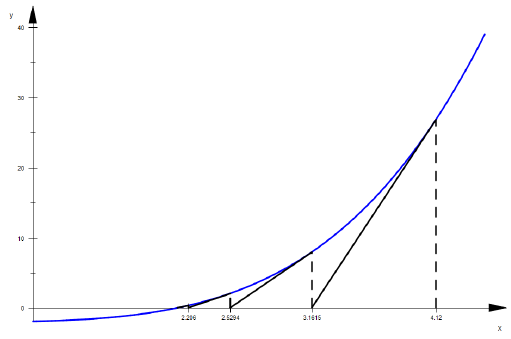
\includegraphics[width=0.6\linewidth]{img/newton_pelda}
		\caption{A Newton-módszer ötlete.}
		\label{fig:newton_pelda}
	\end{figure}
	
	Az ábrán a legszélső, 4.12-es pontból indulunk, felvesszük a függvény ehhez a ponthoz tartozó
	érintőjét, majd ennek az érintőnek a gyöke lesz a következő pont, és így tovább. Általánosan,
	tekintsük az $f$ függvény $x_{k}$ ponthoz tartozó érintőjének egyenletét:
	
	\begin{displaymath}
		y - f(x_{k}) = f'(x_{k}) (x-x_{k})
	\end{displaymath}
	
	\noindent Mint mondtuk, az iteráció $x_{k+1}$. elemét az $x_{k}$-hoz tartozó érintő gyöke adja meg:
	
	\begin{displaymath}
		0 - f(x_{k}) = f'(x_{k}) (x_{k+1}-x_{k}) \Rightarrow
		- \frac{f(x_{k})}{f'(x_{k})} = x_{k+1} - x_{k} \Rightarrow
		x_{k+1} = x_{k} - \frac{f(x_{k})}{f'(x_{k})}
	\end{displaymath}
	
	A fenti képlet a Newton-módszer képlete. Megjegyezhető, hogy a fenti módszer is $x_{k+1} = g(x_{k})$
	alakú (fixpontiteráció).
	
	Fontos megemlíteni, hogy $f'(x_{k}) = 0$ esetén nem értelmezhető a módszer. A gyakorlatban $f'(x_{k}) \approx 0$ is probléma.
	Ha $x^{*}$ többszörös gyök, akkor $f'(x^{*}) = 0$, vagyis $x^{*}$ közelében $f'(x_{k})$ egyre jobban közelít $0$-hoz, numerikusan
	instabil.\\
	
	\noindent \textbf{Monoton konvergencia tétele}: Tegyük fel, hogy $f \in C^{2}[a,b]$ és
	\begin{enumerate}
		\item	$\exists x^{*} \in [a,b] : f(x^{*}) = 0$, azaz van gyök
		
		\item	$f'$ és $f''$ állandó előjelű
		
		\item	$x_{0} \in [a,b]$ legyen olyan, hogy $f(x_{0}) f''(x_{0})) >0$, azaz $f(x_{0}) \not = 0$, valamint $f(x_{0})$ és $f''(x_{0})$
		azonos előjelűek
	\end{enumerate}
	
	\noindent Ekkor az $x_{0}$-ból indított Newton-módszer monoton konvergál $x^{*}$-hoz.
	
	\noindent \textbf{Lokális konvergencia tétele}:	Tegyük fel, hogy $f \in C^{2}[a,b]$ és
	\begin{enumerate}
		\item	$\exists x^{*} \in [a,b] : f(x^{*}) = 0$, azaz van gyök
		
		\item	$f'$ állandó előjelű
		
		\item	$0<m_{1} \leq |f'(x)| (x \in [a,b])$ alsó korlát
		
		\item	$f''(x) \leq M_{2} (x \in [a,b])$ felső korlát, $M:= \frac{M}{2m_{1}}$
		
		\item	$x_{0} \in [a,b]: |x_{0} - x^{*}| < r = \min \left\{\frac{1}{M}, |x^{*}-a|, |x^{*}-b|\right\}$
	\end{enumerate}
	
	\noindent Ekkor az $x_{0}$-ból indított Newton-módszer másodrendben konvergens, hibabecslése:
	
	\begin{displaymath}
		|x_{k+1} - x^{*}| \leq M|x_{0} - x^{*}|^{2}
	\end{displaymath}
	\subsubsection{Húrmódszer}
	
	Továbbra is $f(x) = 0$ megoldása a cél egy adott $[a, b]$ intervallumon. 
	Az eljárás lényege a következő. Kezdetben $x_{0} := a, x_{1} := b$, majd meghúzzuk ezen pontok által
	képzett egyenest. Legyen $x_{2}$ a húr gyöke. Ha $f(x_{2}) = 0$, akkor megtaláltuk a gyököt. Ha $f(x_{2}) \not = 0$,
	akkor folytatjuk a keresést az $[x_{0},x_{2}]$ vagy $[x_{2},x_{1}]$ intervallumban. Ha $f(x_{0})f(x_{2}) < 0$, akkor
	$[x_{0},x_{2}]$ intervallumban folytatjuk, ha $f(x_{2}) f(x_{1}) < 0$, akkor $[x_{2}, x_{1}]$ intervallumban. Stb.
	
	Általánosan: Legyen $x_{0} := a, x_{1} := b$ és	$f(a)f(b) < 0$. Az $(x_{k},f(x_{k}))$ és $(x_{s},f(x_{s}))$
	pontokon átmenő egyenesekkel közelítjük a függvényt	ahol $x_{s}$-re $f(x_{s})f(x_{k})<0$ és $s$ a legnagyobb ilyen index.
	$x_{k+1}$-et a következőképpen határozhatjuk meg:
	
	\begin{displaymath}
		x_{k+1} := x_{k} -
		\frac
		{f(x_{k})}
		{\frac{f(x_{k}) - f(x_{s})}{x_{k}-x_{s}}} =
		x_{k} -
		\frac
		{f(x_{k}) (x_{k} -x_{s}) }
		{f(x_{k}) - f(x_{s})}		
	\end{displaymath}
		
	\noindent \textbf{Tétel}: Legyen $f \in C^{2}[a,b]$ és
	\begin{enumerate}
		\item	$f(a)f(b)<0$
		\item	$M = \frac{M_{2}}{2m_{1}}$, ahol $0<m_{1} \leq |f'(x)|$ és $f''(x) \leq M_{2} (x \in (a,b))$
		\item	$M(b-a) < 1$
	\end{enumerate}
	
	\noindent Ekkor a húrmódszer konvergens, hibabecslése pedig:
	
	\begin{displaymath}
		|x_{k+1} - x^{*}| \leq \frac{1}{M}(M|x_{0}-x^{*}|)^{k+1}
	\end{displaymath}
	
	\subsubsection{Szelőmódszer}
	A szelőmódszer lényege, hogy az $(x_{k},f(x_{k}))$ és $(x_{k-1},f(x_{k-1}))$ pontokon átmenő egyenessel közelítjük
	$f$-et, a kapott egyenes $x$ tengellyel vett metszéspontja $(x_{k+1})$ lesz a következő pont. Ez
	tulajdonképpen a húrmódszer $s := k - 1$-re.
	
	\begin{displaymath}
		x_{k+1} :=
		x_{k} -
		\frac
		{f(x_{k}) (x_{k} -x_{k-1}) }
		{f(x_{k}) - f(x_{k-1})}		
	\end{displaymath}
	
	\noindent \textbf{Tétel}: Ha teljesülnek a Newton-módszer lokális konvergencia tételének feltételei, akkor a szelőmódszer
	konvergens $p = \frac{1+\sqrt{5}}{2}$ rendben ,és hibabecslése:
	
	\begin{displaymath}
		|x_{k+1} - x^{*}| \leq M|x_{k}-x^{*}||x_{k-1}-x^{*}|
	\end{displaymath}
	
	\subsubsection{Többváltozós Newton-módszer}
	
	Most $F(x) = 0$ megoldásait keressük, ahol $F \in \mathbb{R}^{n} \to \mathbb{R}^{n}$. Tekintsük a többváltozós Newton-módszert:
	
	\begin{displaymath}
		x^{(k+1)} := x^{(k)} - [F'(x^{(k)})]^{-1}F(x^{(k)})
	\end{displaymath}
	
	\noindent ahol
	
	\begin{displaymath}
		F(x) = \begin{bmatrix}
		f_{1}(x) \\[0.3em]
		f_{2}(x) \\[0.3em]
		...  \\[0.3em]
		f_{n}(x)
		\end{bmatrix},
		F'(x) = \begin{bmatrix}
		\partial_{1}f_{1}(x) & \partial_{2}f_{1}(x)& ... \\[0.3em]
		\partial_{1}f_{2}(x) & \partial_{2}f_{2}(x)& ... \\[0.3em]
		... & ... & ...
		\end{bmatrix}
	\end{displaymath}
	
	\noindent Ténylegesen az $F'(x^{(k)}) (x^{(k+1)} - x^{(k)}) = -F(x^{(k)})$ egyenletrendszert oldjuk meg.
	
	\section{Interpoláció}
	
	A gyakorlatban sokszor felmerül olyan probléma, hogy egy többségében ismeretlen (csak néhány pontbeli érték ismert) 
	vagy nagyon költségesen kiszámítható függvénnyel kellene egy megadott intervallumon dolgoznunk.
	Ekkor például azt tehetjük, hogy néhány pontban kiszámítjuk	a függvény értékét, 
	majd keresünk olyan egyszerűbben számítható függvényt, amelyik illeszkedik az
	adott pontokra. Ezután az intervallum bármely további pontjában az illesztett függvény értékeit használjuk, mint
	az eredeti függvény értékeinek a közelítéseit. Ilyen egyszerűbben kiszámolható függvények pl. a polinomok (polinom interpoláció).
	
	Példa alkalmazásra: Animáció készítésénél nem szeretnénk minden egyes képkockát saját magunk elkészíteni, hanem csak bizonyos képkockákat,
	ún. kulcskockákat. A köztes képkockákon az egyes objektumok helyzetét szeretnénk a számítógéppel kiszámíttatni (például szeretnénk, hogy
	ha egy objektum egyenes vonalú, egyenletes mozgást végezne két adott pozíció között).
	
	\subsection{Polinom interpoláció}
	
	\subsubsection{A polinom interpoláció feladata}
	Legyenek adva $n \in \mathbb{N}$ és az $x_{k} \in \mathbb{R}, k=0,1,..,n$ különböző számok, az ún. interpolációs alappontok, valamint
	az $f(x_{k}),k=0,1,..,n$ számok, az ismert függvényértékek. Keressük azt a legfeljebb $n$-edfokú $p_{n}$ polinomot $(p_{n} \in P_{n})$,
	amelyre:
	
	\begin{displaymath}
		p_{n}(x_{k}) = f(x_{k}) \ \ k=0,1,...,n
	\end{displaymath}
	
	\noindent Azaz a keresett polinom az interpolációs alappontokban a megadott függvényértékeket veszi fel.\\
	
	\noindent \textbf{Tétel}: A fenti interpolációs feladatnak egyértelműen létezik megoldása.\\
	
	\subsubsection{Lagrange-interpoláció}
	Az interpolációs polinom kiszámolására explicit képletet ad a Lagrange-interpoláció.\\
	
	\noindent \textbf{Lagrange-alappolinomok}: Adott $n \in \mathbb{N}$ és $x_{k} \in \mathbb{R}, k=0,1,...,n$ különböző alappontokra
	a Lagrange-alappolinomokat a következőképpen definiáljuk:
	
	\begin{displaymath}
		l_{k}(x) =
		\frac
		{\displaystyle\prod_{\substack{j=0\\j \not = k}}^{n}(x-x_{j})}
		{\displaystyle\prod_{\substack{j=0\\j \not = k}}^{n}(x_{k}-x_{j})}
	\end{displaymath}
	
	\noindent $k=0,1, ..., n$ esetén.\\
	
	\noindent Az alappontok mind $n$-edfokú polinomok, és a következő tulajdonsággal rendelkeznek:
	
	\begin{displaymath}
		l_{k}(x_{j})=\left\{\begin{array}{lr}
		1 & ha \ j=k \\
		0 & ha \ j \not = k
		\end{array}
		\right\}
	\end{displaymath}
	
	\noindent \textbf{Tétel}: Az interpolációs feladat megoldása az alábbi polinom, amelyet az interpolációs
	polinom Lagrange-alakjának hívunk:
	
	\begin{displaymath}
		L_{n}(x) = \sum_{k=0}^{n}f(x_{k})l_{k}(x)
	\end{displaymath}
	
	\noindent A továbbiakban jelölje $[a,b]$ az $x_{0}, x_{1}, ..., x_{n}$ alappontok által kifeszített intervallumot.\\
	
	\noindent \textbf{A Lagrange-interpoláció hibája}: Ha $f \in C^{n+1}[a,b]$, akkor $\forall x \in [a,b]$ esetén
	\begin{displaymath}
		|f(x) - L_{n}(x)| \leq \frac{M_{n+1}}{(n+1)!}|\omega_{n}(x)|
	\end{displaymath}
	
	\noindent ahol $\omega_{n}(x) = \displaystyle\prod_{i=0}^{n}(x-x_{i})$, valamint $M_{k} = \displaystyle\max_{[a,b]}|f^{(k)}(x)|$.\\
	
	\noindent \textbf{Egyenletes konvergencia}: Legyen $f \in C^{\infty}[a,b]$ és legyen adva egy $[a,b]$ intervallumbeli
	alappontrendszerek sorozata: $x_{k}^{(n)}$, $k=0,1,...,n$, $n=0,1,2,...$. Legyen $L_{n}$ az $x_{0}^{(n)}, ... ,x_{n}^{(n)}$
	alappontrendszerre illesztett Lagrange-interpolációs polinom ($n=0,1,2,...$). Ekkor ha $\exists M>0$ úgy, hogy
	$M_{n} \leq M^{n} \ \forall n \in \mathbb{N}$, akkor az $L_{n}$ sorozat egyenletesen konvergál az $f$ függvényhez.\\

	\noindent \textbf{Marcinkiewicz tétele}: Minden $f \in C[a,b]$ esetén létezik a fenti módon definiált alappontrendszer
	úgy, hogy $\Vert f - L_{n}\Vert_{\infty} \to 0$.\\
	
	\noindent \textbf{Faber tétele}: Minden a fenti módon definiált alappontrendszer esetén van olyan $f \in C[a,b]$ függvény,
	hogy $\Vert f - L_{n}\Vert_{\infty} \not \to 0$.\\

	\noindent \textbf{Osztott differencia}: Legyenek adva az $x_{k} \in [a,b], k=0,1,...,n$ különböző alappontok.
	Az $f:[a,b] \to \mathbb{R}$ függvénynek a megadott alappontrendszerre vonatkozó elsőrendű osztott differenciái
	
	\begin{displaymath}
		f[x_{i},x_{i+1}] = \frac{f(x_{i+1})-f(x_{i})}{x_{i+1} - x_{i}}
	\end{displaymath}
	
	\noindent a magasabb rendű osztott differenciákat rekurzívan definiáljuk. Tegyük fel, hogy a $k-1$ rendű osztott differenciák
	már definiálva lettek, akkor a $k$-adrendű osztott differenciák az alábbiak:
	
	\begin{displaymath}
		f[x_{i},x_{i+1},...,x_{i+k}] = \frac{f[x_{i+1},x_{i+2}, ..., x_{i+k}]-f[x_{i},x_{i+1}, ..., x_{i+k-1})]}{x_{i+k} - x_{i}}
	\end{displaymath}
	
	\noindent Látható, hogy a $k$-adrenű osztott differencia $k+1$ alappontra támaszkodik.\\
	
	Ha adott egy interpoláció alappontrendszer függvényértékekkel, akkor a hozzá tartozó osztott differenciákat az
	alábbi táblázat szerint érdemes elrendezni, és ez az elrendezés egyúttal a kiszámolást is segíti.
	
	\begin{table}[H]
		\begin{tabular}{llllllll}
			$x_{0}$ & $f(x_{0})$ &  &  &  &  & & \\ 
			$x_{1}$ & $f(x_{1})$ & $f[x_{0},x_{1}]$ &  &  &  & & \\
			$x_{2}$ & $f(x_{2})$ & $f[x_{1},x_{2}]$ &  &  &  &  &\\
			\rotatebox[origin=c]{90}{...} & \rotatebox[origin=c]{90}{...}&  &  &  &  &  &\\
			$x_{k}$& $f(x_{k})$ & $f[x_{k-1},x_{k}]$ & ... &  $f[x_{0}, x_{1}, ..., x_{k}]$ &  & & \\
			\rotatebox[origin=c]{90}{...} &\rotatebox[origin=c]{90}{...}  &  & &  &  & & \\
			$x_{n-1}$ & $f(x_{n-1})$ & $f[x_{n-2},x_{n-1}]$  & ... &  $f[x_{n-1-k}, x_{n-k}, ..., x_{n-1}]$& ... &
			$f[x_{0}, x_{1}, ..., x_{n-1}]$ &\\
			$x_{n} $& $f(x_{n})$ & $f[x_{n-1},x_{n}]$ & ... &  $f[x_{n-k}, x_{n-k+1}, ..., x_{n}]$ & ... &
			$f[x_{1}, x_{2}, ..., x_{n}]$ & $f[x_{0}, x_{1}, ..., x_{n}]$\\
		\end{tabular}
	\end{table}
	
	
	\noindent \textbf{Az interpolációs polinom Newton-alakja}: Az interpolációs polinom az alábbi alakban felírható:
	\begin{displaymath}
		N_{n}(x) = f(x_{0}) + \displaystyle\sum_{k=1}^{n}f[x_{0},x_{1}, ..., x_{k}] \omega_{k-1}(x)
	\end{displaymath}
	
	\noindent ahol $\omega_{j}(x) =  (x-x_{0})(x-x_{1})...(x-x_{j})$. Ezt az alakot az interpolációs polinom Newton-alakjának hívjuk.
	
	\subsubsection{Hermite-interpoláció}
	Az előbbi interpolációs feladatot a következőképpen általánosíthatjuk. Legyenek adva az egyes alappontokban a függvényértékek
	mellett a függvény derivált értékei is valamely rendig bezárólag. Ekkor olyan polinomot keresünk, amelyik deriváltjaival együtt
	illeszkedik a megadott értékekre, vagyis:\\
	
	\noindent Legyenek adva $n,m_{0},m_{1},..., m_{n} \in \mathbb{N}$ és az $x_{j} \in \mathbb{R}, j=0,1,...,n$ interpolációs
	alappontok, valamint az $f^{(k)}(x_{j}) \ \ k=0,1,...,m_{j}-1, \ \ \ j=0,1,...,n$ függvény- és derivált értékek. Legyen
	$m = \displaystyle\sum_{j=0}^{n}m_{j}$ Keressük azt a legfeljebb ($m-1$)-edfokú $p_{m-1}$ polinomot, melyre:
	
	\begin{displaymath}
		p^{(k)}_{m-1}(x_{j}) = f^{(k)}(x_{j}) \ \ k=0,1,...,m_{j}-1, \ \ \ j=0,1,...,n
	\end{displaymath}
	
	\noindent \textbf{Megjegyzések}:
	\begin{enumerate}
		\item	Ha $m_{j}=2, j=0,1,...,n$, akkor a feladatot Hermite-Fejér-féle interpolációnak nevezzük. Ekkor minden alappontban
		a függvény- és az első derivált érték adott. A keresett polinom pedig legfeljebb ($2n+1$)-edfokú.
		
		\item	Ha $m_{j}=1, j=0,1,...,n$, akkor a Lagrange-interpolációt kapjuk vissza.
	\end{enumerate}
	
	\noindent \textbf{Osztott differencia ismétlődő allapontokra}: Ha $x_{k}$ $j$-szer szerepel:
	\begin{displaymath}
		f[x_{k}, ... x_{k}] = \frac{f^{(j)}(x_{k})}{j!}
	\end{displaymath}
	
	\noindent \textbf{Tétel}: A Hermite-féle interpolációs polinom egyértelműen létezik.\\
	
	\noindent \textbf{A Hermite interpolációs polinom előállítása}: Könnyen felírható a Newton-féle formában. Csak annyit
	kell tennünk, hogy kiindulunk az alappontok és a függvényértékek táblázatával és legyártjuk az osztott differenciák
	táblázatát. Az az egyetlen különbség most, hogy az $x_{j}$ alappontot $m_{j}$-szer soroljuk fel.\\
	
	\noindent \textbf{Hermite-interpoláció hibája}: Ha $f \in C^{m}[a,b]$, akkor $\forall x \in [a,b]:$
	
	\begin{displaymath}
		|f(x) - H_{m-1}(x)| \leq \frac{M_{m}}{m!}|\Omega_{m}(x)|
	\end{displaymath}
	
	\noindent ahol $\Omega_{m}(x) = (x-x_{0})^{m_{0}}(x-x_{1})^{m_{1}}...(x-x_{n})^{m_{n}}$
	
	\subsection{Spline-interpoláció}
	
	Az eddig említett interpolációs módszerekben polinomokkal dolgoztunk. Lehetőség van arra is, hogy a megadott pontrendszerre más
	típusú függvényt próbáljunk illeszteni. Igen előnyös tulajdonságokkal rendelkeznek a bizonyos folytonossági előírásoknak is
	megfelelő, szakaszonként polinom függvények, a spline-ok.\\
	
	\noindent \textbf{$l$-edfokú spline}: Legyen adott $\Omega_{n} = \left\{x_{0}, x_{1}, ..., x_{n}\right\}$ az $[a,b]$ intervallum egy
	felosztása, ahol $x_{0}=a, x_{n}=b$ és $l \in \mathbb{N}$. Az $s:[a,b] \to \mathbb{R}$ függvény egy $l$-edfokú spline az
	$\Omega_{n}$-re vonatkozóan, ha:
	
	\begin{enumerate}
		\item	$s_{|[x_{k-1},x_{k}]}$ egy $l$-edfokú polinom $\forall k = 1,..,n$
		
		\item	$s \in C^{l-1}[a,b]$, tehát a teljes intervallumon $(l-1)$-szer folytonosan derviálható
	\end{enumerate}
	
	\noindent Jelölés: $s_{l}(\Omega_{n})$ az $\Omega_{n}$-hez tartozó $l$-edfokú spline-ok halmaza.\\
	
	\noindent \textbf{Spline-interpoláció}: Legyenek adottak $x_{k},f(x_{k})$ értékek $k=0,1,..,n$-re és $l \in \mathbb{N}$.
	Keressük azt az $s \in s_{l}(\Omega_{n})$ spline-t, amelyre $s(x_{k}) = f(x_{k})$. Ehhez elő kell állítanunk minden
	intervallumra egy $l$-edfokú polinomot. Ha a polinomokat az együtthatóikkal reprezentáljuk, akkor ez $n(l+1)$ ismeretlen.
	Az előírt feltételek száma: $2n$ interpolációs és $(l-1)(n-1)$ folytonossági feltétel, hiszen csak a belső pontokban kell
	előírni az illető deriváltakra vonatkozó megfelelő folytonossági feltételt. Az így kapott összes feltétel darabszáma
	$(l+1)n - (l-1)$, tehát az egyértelműséghez $l-1$ feltétel hiányzik még. Ezeket úgynevezett peremfeltételekkel adjuk meg.
	Pl. a harmadfokú spline-interpolációhoz 2 peremfeltétel szükséges. Ezek a következők (ezek közül elég egyet választani,
	mert mindegyik 2 feltételt tartalmaz):
	
	\begin{enumerate}
		\item	Természetes peremfeltétel: $s''(a) = s''(b) = 0$.
		
		\item	Hermite-féle peremfeltétel: $s'(a) = s_{a}, s'(b) = s_{b}$, ahol $s_{a}, s_{b}$ előre megadott számok.
		
		\item	Periodikus peremfeltétel (ekkor feltételezzük, hogy $s(a) = s(b)$ is teljesül):
		$s'(a) = s'(b)$ és $s''(a) = s''(b)$
	\end{enumerate}
	
	\noindent \textbf{Elsőfokú spline előállítása}: Az elsőfokú spline előállítása triviális szakaszonkénti
	lineáris Lagrange-interpolációval.\\
	
	\noindent \textbf{Másodfokú spline előállítása}: Egyetlen peremfeltétel szükséges, legyen a következő: $s'(a) = s_{a}$
	valamilyen $s_{a}$ számra. Az $[x_{0},x_{1}]$ szakaszon Hermite-interpolációval előállítjuk azt a $H_{2}$ másodfokú
	polinomot, amely megfelel az interpolációs feltételeknek és a peremfeltételnek. Az így kapott polinom $x_{1}$-beli
	deriváltja meghatározott, tehát a folytonos deriválhatóság miatt az $[x_{1},x_{2}]$ szakaszon a bal végpontban
	adott a derivált értéke. Ismét Hermite-interpolációt alkalmazva megkapjuk az $[x_{1},x_{2}]$ szakaszhoz tartozó
	polinomot. Ezt az eljárást ismételve állíthatjuk elő a másodfokú interpolációs spline-t.\\
	
	\noindent \textbf{Függvény tartója}: A $supp(f) := \overline{\left\{x \in \mathbb{R}: f(x) \not = 0 \right\}}$ halmazt
	az $f$ függvény tartójának nevezzük.\\
	
	\noindent \textbf{Számegyenes felosztása}: $\Omega_{\infty} := \left\{...,x_{-2},x_{-1},x_{0},x_{1},...x_{n},x_{n+1},...\right\}$\\
	
	\noindent \textbf{B-spline}: A $B_{l,k}, k \in \mathbb{Z}$ $l$-edfokú spline függvények rendszerét B-spline függvényeknek
	nevezzük, ha az alábbi feltételek teljesülnek:
	\begin{enumerate}
		\item	$supp(B_{l,k}) = [x_{k},x_{k+l+1}]$, azaz a tartója minimális
		
		\item	$B_{l,k}(x) \geq 0$
		
		\item	$\displaystyle\sum_{k \in \mathbb{Z}}B_{l,k}(x) = 1$
	\end{enumerate}
	
	\section{Legkisebb négyzetek módszere}
	
	Gyakorlati feladatok során adódik a következő probléma. Egy elsőfokú függvényt mérünk bizonyos pontokban, de
	a mérési hibák miatt ezek nem lesznek egye egyenesen. Ekkor olyan egyenest keresünk, amelyik az alábbi
	értelemben legjobban illeszkedik a megadott mérési ponthalmazra.
	
	Legyenek adva az $(x_{i},y_{i}), i=1,2,..,m$ mérési pontok. Keressük azt a $p_{1}(x) = a + bx$ legfeljebb
	elsőfokú polinomot, amelyre a
	
	\begin{displaymath}
		\displaystyle\sum_{i=1}^{m}(y_{i}-p_{1}(x_{i}))^{2} =
		\displaystyle\sum_{i=1}^{m}(y_{i}- a - bx_{i})^{2}
	\end{displaymath} 

	\noindent kifejezés minimális. Ez azt jelenti, hogy azt az egyenes keressük, amelyre a függvényértékek hibáinak
	négyzetösszege minimális.
	
	Az általános feladat az alábbi.
	
	Adottak az $m,n \in \mathbb{N}$, ahol $m >> n$ és $(x_{i},y_{i}), i= 1,2,...,m$ mérési pontok, ahol az $x_{i}$
	alappontok különbözők. Keressük azt a $p_{n}(x) = a_{0} + a_{1}x + ... a_{n}x^{n}$ legfeljebb $n$-edfokú
	polinomot, melyre a

	\begin{displaymath}
	\displaystyle\sum_{i=1}^{m}(y_{i}-p_{n}(x_{i}))^{2}
	\end{displaymath} 
	
	\noindent kifejezés minimális.
	
	A feladat megoldásához tekintsük annak egy átfogalmazását.
	
	Vegyük a $p_{n}(x_{i}) = y_{i}, i=1,2,...,m)$ egyenletrendszert. Ez a rendszer az ismeretlen $a_{i}$ együtthatókra nézve
	lineáris, mégpedig túlhatározott, amelynek az $A$ mátrixa egy téglalap alakú Vandermonde-mátrix $A \in \mathbb{R}^{m \times (n+1)}$,
	a $b \in \mathbb{R}^{m}$ jobb oldali vektora pedig a függvényértékekből adódik:
	
	\begin{displaymath}
	\begin{bmatrix}
	1 & x_{1} & x_{1}^{2} & ... & x_{1}^{n} \\[0.3em]
	1 & x_{2} & x_{2}^{2} & ... & x_{2}^{n} \\[0.3em]
	1 & x_{3} & x_{3}^{2} & ... & x_{3}^{n} \\[0.3em]
	\rotatebox[origin=c]{90}{...} & \rotatebox[origin=c]{90}{...} &\rotatebox[origin=c]{90}{...} & \rotatebox[origin=c]{90}{...} & \rotatebox[origin=c]{90}{...} \\[0.3em]
	1 & x_{m} & x_{m}^{2} & ... & x_{m}^{n} \\[0.3em]
	\end{bmatrix}
	\begin{bmatrix}
	a_{0} \\[0.3em]
	a_{1} \\[0.3em]
	a_{2} \\[0.3em]
	\rotatebox[origin=c]{90}{...} \\[0.3em]
	a_{n}
	\end{bmatrix}
	=
	\begin{bmatrix}
	y_{0} \\[0.3em]
	y_{1} \\[0.3em]
	y_{2} \\[0.3em]
	\rotatebox[origin=c]{90}{...} \\[0.3em]
	y_{m}
	\end{bmatrix}
	\end{displaymath}
	
	Ezen jelölésekkel a minimalizálandó kifejezés $\Vert Az - b \Vert_{2}^{2}$, ahol $z = [a_{0},a_{1}, ..., a_{n}]^{T}$
	a keresett együtthatók vektora. A feladat megoldását a Gauss-féle normálegyenletek adják:
	
	\begin{displaymath}
		A^{T}Az = A^{T}b
	\end{displaymath}
	
	\noindent A fenti LER-t kell megoldani $z$-re.\\
	
	\noindent \textbf{n=1 eset}: Ekkor a feladatot gyakran lineáris regressziónak is hívjuk. Ebben az esetben
	\begin{displaymath}
		A^{T}A = \begin{bmatrix}
		m & \sum_{i=1}^{m} x_{i} \\[0.3em]
		\sum_{i=1}^{m} x_{i} & \sum_{i=1}^{m} x_{i}^{2}
		\end{bmatrix} \ ,
		A^{T}b = \begin{bmatrix}
		\sum_{i=1}^{m} y_{i} \\[0.3em]
		\sum_{i=1}^{m} x_{i}y_ {i} 
		\end{bmatrix} \ ,
		z= \begin{bmatrix}
		b \\[0.3em]
		a
		\end{bmatrix}
	\end{displaymath}
	
\end{document}